\documentclass{article}
\usepackage[utf8]{inputenc}
% are all of these packages really necessary?
% no.
% i'm just too lazy to only grab the packages i want for a specific
% document, so i just glob all of my most commonly used packages together
% this is bad practice.
\usepackage{amsmath,amsthm,amssymb,amsfonts, fancyhdr, color, comment, graphicx, environ, mdframed, soul, calc, enumitem, mdframed, xcolor, geometry, empheq, mathtools, tikz, pgfplots, caption, subcaption, hyperref}

\usetikzlibrary{external}
\tikzexternalize[prefix=tikz/,optimize command away=\includepdf]

%tikzpicture
\usepackage{tikz}
\usepackage{scalerel}
\usepackage{pict2e}
\usepackage{tkz-euclide}
\usetikzlibrary{calc}
\usetikzlibrary{patterns,arrows.meta}
\usetikzlibrary{shadows}
\usetikzlibrary{external}

%pgfplots
\usepackage{pgfplots}
\pgfplotsset{compat=newest}
\usepgfplotslibrary{statistics}
\usepgfplotslibrary{fillbetween}
\usepgfplotslibrary{polar}

\tikzset{external/export=true}
\pgfplotsset{
    standard/.style={
    axis line style = thick,
    trig format=rad,
    enlargelimits,
    axis x line=middle,
    axis y line=middle,
    enlarge x limits=0.15,
    enlarge y limits=0.15,
    every axis x label/.style={at={(current axis.right of origin)},anchor=north west},
    every axis y label/.style={at={(current axis.above origin)},anchor=south east}
    }
}
\newcommand*\widefbox[1]{\fbox{\hspace{2em}#1\hspace{2em}}}
% Command "alignedbox{}{}" for a box within an align environment
% Source: http://www.latex-community.org/forum/viewtopic.php?f=46&t=8144
\newlength\dlf  % Define a new measure, dlf
\newcommand\alignedbox[2]{
% Argument #1 = before & if there were no box (lhs)
% Argument #2 = after & if there were no box (rhs)
&  % Alignment sign of the line
{
\settowidth\dlf{$\displaystyle #1$}  
    % The width of \dlf is the width of the lhs, with a displaystyle font
\addtolength\dlf{\fboxsep+\fboxrule}  
    % Add to it the distance to the box, and the width of the line of the box
\hspace{-\dlf}  
    % Move everything dlf units to the left, so that & #1 #2 is aligned under #1 & #2
\boxed{#1 #2}
    % Put a box around lhs and rhs
}
}

\hypersetup{
    colorlinks=true,
    linkcolor=blue,
    filecolor=magenta,      
    urlcolor=cyan,
    pdftitle={Homework 21 Solutions},
    pdfpagemode=UseOutlines,
    bookmarksopen=true,
    pdfauthor={Christina Phan}
}
\newcommand{\lrp}[1]{\left( #1 \right)}
\newcommand{\abs}[1]{\left\vert #1 \right\vert}
\newcommand{\lra}[1]{\left\langle #1 \right\rangle}
\newcommand{\lrb}[1]{\left[ #1 \right]}
\newcommand{\norm}[1]{\left\lVert #1 \right\rVert}
\newcommand{\iintR}[0]{\iint\limits_{R}}
\renewcommand{\u}[0]{\mathbf{u}}
\renewcommand{\i}[0]{\mathbf{i}}
\renewcommand{\j}[0]{\mathbf{j}}
\renewcommand{\k}[0]{\mathbf{k}}
\newcommand{\T}[0]{\mathbf{T}}
\newcommand{\N}[0]{\mathbf{N}}
\newcommand{\B}[0]{\mathbf{B}}
\renewcommand{\r}[0]{\mathbf{r}}
\renewcommand{\a}[0]{\mathbf{a}}
\renewcommand{\v}[0]{\mathbf{v}}
\newcommand{\F}[0]{\mathbf{F}}
\newcommand{\n}[0]{\mathbf{n}}
\newcommand{\eqq}[0]{\stackrel{?}{=}}
\renewcommand{\arraystretch}{1.25}

\geometry{letterpaper, portrait, margin=1in}
\renewcommand{\footrulewidth}{0.8pt}
\setlength\parindent{0pt}
\pagestyle{fancy}
\lhead{Christina Phan}
\rhead{MAT 21D} 
\chead{\textbf{Homework 21 Solutions}}

\newcommand{\Solution}{\textit{Solution}}
\pgfplotsset{compat=1.18}
\begin{document}

\phantomsection
\addcontentsline{toc}{section}{Problem 1 (Parts)}\textbf{Problem 1 (Parts)}

Find the curl of the vector field:

\phantomsection
\addcontentsline{toc}{subsection}{1(a)}\textbf{(a)} $\F(x,y,z)=\lra{xy+z,yz+x,xz+y}$

\Solution

Recall that the curl of a vector field $\F$ is
\begin{equation*}
    \text{curl}=\nabla \times \F
\end{equation*}
Let's find the curl for $\F(x,y,z)=\lra{xy+z,yz+x,xz+y}$.
\begin{align*}
    \text{curl}&=\nabla \times \F \\
    &=\begin{vmatrix}
    \i & \j & \k \\
    \frac{\partial }{\partial x} &  \frac{\partial }{\partial y} &
     \frac{\partial }{\partial z}\\
     xy+z & yz+x& xz+y
    \end{vmatrix}\\
    &=\Bigg(\frac{\partial }{\partial y}(xz+y)-\frac{\partial }{\partial z}(yz+x)\Bigg)\i-\Bigg(\frac{\partial}{\partial x}(xz+y)-\frac{\partial}{\partial z}(xy+z)\Bigg)\j+\Bigg(\frac{\partial}{\partial x}(yz+x)-\frac{\partial}{\partial y}(xy+z)\Bigg)\k\\
    &=\lrp{1-y}\i-\lrp{z-1}\j+\lrp{1-x}\k\\
    &=\lrp{1-y}\i-\lrp{z-1}\j+\lrp{1-x}\k\\
    &=\lrp{1-y}\i+\lrp{-z+1}\j+\lrp{1-x}\k\\
    &=\boxed{\lra{1-y,1-z,1-x}}
\end{align*}

\phantomsection
\addcontentsline{toc}{subsection}{1(b)}\textbf{(b)} $\F(x,y,z)=\lra{ye^z,ze^x,-xe^y}$

\Solution

Recall that the curl of a vector field $\F$ is
\begin{equation*}
    \text{curl}=\nabla \times \F
\end{equation*}
Let's find the curl for $\F(x,y,z)=\lra{ye^z,ze^x,-xe^y}$.
\begin{align*}
     \text{curl}&=\nabla \times \F\\ &=\begin{vmatrix}
    \i & \j & \k \\
    \frac{\partial }{\partial x} &  \frac{\partial }{\partial y} &
     \frac{\partial }{\partial z}\\
     ye^z & ze^x& -xe^y
    \end{vmatrix}\\
    &=\Bigg(\frac{\partial }{\partial y}(-xe^y)-\frac{\partial }{\partial z}(ze^x)\Bigg)\i-\Bigg(\frac{\partial}{\partial x}(-xe^y)-\frac{\partial}{\partial z}(ye^z)\Bigg)\j+\Bigg(\frac{\partial}{\partial x}(ze^x)-\frac{\partial}{\partial y}(ye^z)\Bigg)\k\\
    &=\lrp{-xe^y-e^x}\i-\lrp{-e^y-ye^z}\j+\lrp{ze^x-e^z}\k\\
    &=\lrp{-xe^y-e^x}\i+\lrp{e^y+ye^z}\j+\lrp{ze^x-e^z}\k\\
    &=\boxed{\lra{-xe^y-e^x,e^y+ye^z,ze^x-e^z}}
\end{align*}

\phantomsection
\addcontentsline{toc}{subsection}{1(c)}\textbf{(c)} $\F(x,y,z)=\nabla f$, where $f(x,y,z)$ has continuous second partial derivatives

\Solution

Recall that the curl of a vector field $\F$ is
\begin{equation*}
    \text{curl}=\nabla \times \F
\end{equation*}
Let's find the curl for $\displaystyle \F(x,y,z)=\nabla f = \lra{\frac{\partial f}{\partial x}, \frac{\partial f}{\partial y},\frac{\partial f}{\partial z}}$.
\begin{align*}
     \text{curl}&=\nabla \times \F\\ &=\begin{vmatrix}
    \i & \j & \k \\
    \frac{\partial }{\partial x} &  \frac{\partial }{\partial y} &
     \frac{\partial }{\partial z}\\
     \frac{\partial f}{\partial x} & {\frac{\partial f}{\partial y}} & {\frac{\partial f}{\partial z}}
    \end{vmatrix}\\
    &=\Bigg(\frac{\partial }{\partial y}\lrp{\frac{\partial f}{\partial z}}-\frac{\partial }{\partial z}\lrp{\frac{\partial f}{\partial y}}\Bigg)\i-\Bigg(\frac{\partial}{\partial x}\lrp{\frac{\partial f}{\partial z}}-\frac{\partial}{\partial z}\lrp{\frac{\partial f}{\partial x}}\Bigg)\j+\Bigg(\frac{\partial}{\partial x}\lrp{\frac{\partial f}{\partial y}}-\frac{\partial}{\partial y}\lrp{\frac{\partial f}{\partial x}}\Bigg)\k\\
    &=\Bigg(\frac{\partial ^2f}{\partial y\partial z}-\frac{\partial^2f}{\partial z\partial y}\Bigg)\i-\Bigg(\frac{\partial ^2f}{\partial x\partial z}-\frac{\partial^2f}{\partial z\partial x}\Bigg)\j+\Bigg(\frac{\partial ^2f}{\partial x\partial y}-\frac{\partial^2f}{\partial y\partial x}\Bigg)\k\\
    &=\Bigg(\frac{\partial ^2f}{\partial y\partial z}-\frac{\partial^2f}{\partial y\partial z}\Bigg)\i-\Bigg(\frac{\partial ^2f}{\partial x\partial z}-\frac{\partial^2f}{\partial x\partial z}\Bigg)\j+\Bigg(\frac{\partial ^2f}{\partial x\partial y}-\frac{\partial^2f}{\partial x\partial y}\Bigg)\k\tag{See Note}\\
    &=\lrp{0}\i-\lrp{0}\j+\lrp{0}\k\\
    &=\boxed{\lra{0,0,0}}
\end{align*}
\textbf{Note}

Since we know $f(x,y,z)$ has continuous second partial derivatives, we know that the mixed second derivatives are equal. This might have been covered in MAT 21C and/or MAT 21D. Feel free to PM me for a proof on it!

\phantomsection
\addcontentsline{toc}{section}{Problem 2 (Parts)}\textbf{Problem 2 (Parts)}

Use Stokes' Theorem to find $\displaystyle \int_C \F\cdot \,d\r$ counterclockwise around the curve $C$:

\phantomsection
\addcontentsline{toc}{subsection}{2(a)}\textbf{(a)} $\F(x,y,z)=\lra{2y,3x,-z^2}$, $C$ is the circle $x^2+y^2=9$.

\Solution

To find what $\displaystyle\iint_S \lrp{\nabla \times \F}\cdot \n\,d\sigma$, we'll need to know what $\nabla \times \F$ is and what $\n\,d\sigma$ is.

\phantomsection
\addcontentsline{toc}{subsubsection}{Curl} \textbf{Curl ($\displaystyle\nabla \times \F$)}

Since $\F(x,y,z)=\lra{2y,3x-z^2}$,
\begin{align*}
    \nabla \times \F &=\begin{vmatrix}
    \i & \j & \k \\
    \frac{\partial }{\partial x} &  \frac{\partial }{\partial y} &
     \frac{\partial }{\partial z}\\
     2y& 3x & -z^2
    \end{vmatrix}\\
    &=\Bigg(\frac{\partial }{\partial y}(-z^2)-\frac{\partial }{\partial z}(3x)\Bigg)\i-\Bigg(\frac{\partial}{\partial x}(-z^2)-\frac{\partial}{\partial z}(2y)\Bigg)\j+\Bigg(\frac{\partial}{\partial x}(3x)-\frac{\partial}{\partial y}({2y})\Bigg)\k\\
    &=\lrp{0-0}\i-\lrp{0-0}\j +\lrp{3-2}\k\\
    &=\lrp{0}\i-\lrp{0}\j+\lrp{1}\k\\
    &=\lra{0,0,1}
\end{align*}

\phantomsection
\addcontentsline{toc}{subsubsection}{n dsigma} \textbf{$\n\,d\sigma$}


Please see today's (5/23) lecture recording if this explanation is not sufficient.

Since our curve $C$ is just on the $xy$-plane, we know $\n=\k=\lra{0,0,1}$ and $d\sigma = dA$. Therefore,
\begin{equation*}
    \n\,d\sigma =\lra{0,0,1}\,dA
\end{equation*}

t
\begin{align*}
    \iint_C \F\cdot d\r&=\iint_S\lrp{\nabla \times \F}\cdot \n \,d\sigma = \iint_R \lra{0,0,1}\cdot \lra{0,0,1}\,dA
\end{align*}
Our region $R$ (the shadow of the surface on the $xy$-plane) is $x^2+y^2=9$. Graphically, this looks like
\begin{center}
\resizebox{3.5cm}{!}{
    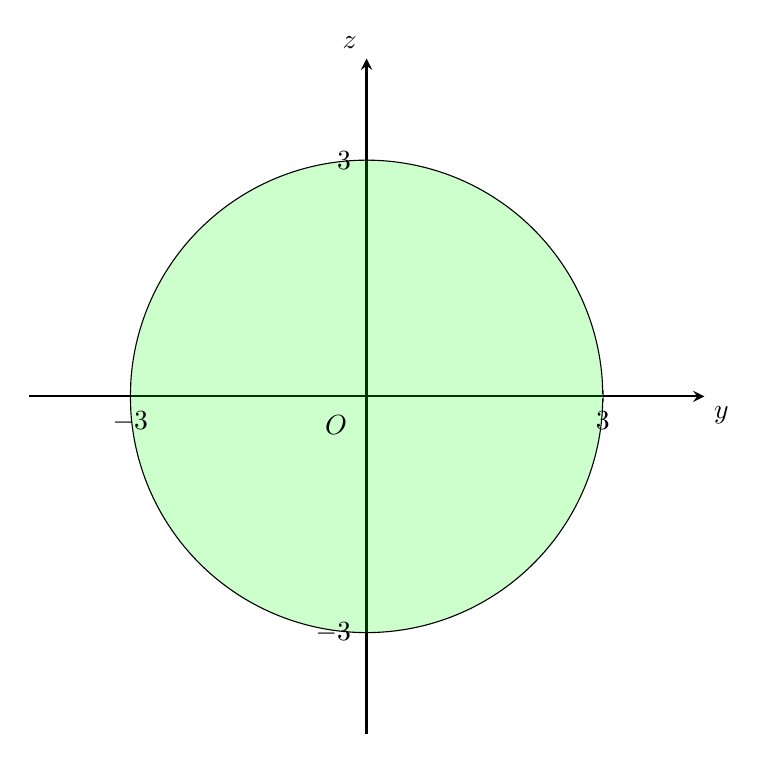
\begin{tikzpicture}
    \begin{axis}[standard,
            xtick={-3,3},
            ytick={-3,3},
            samples=1000,
            xlabel={$y$},
            ylabel={$z$},
          xmin=-3.3,
          xmax=3.3,          
          ymin=-3.3,
          ymax=3.3,
            x=1cm,
            y=1cm/1,
           ]

    \node[anchor=center,label=south west:$O$] at (axis cs:0,0){};
\addplot[name path=F,domain={-3:3}]{sqrt(9-x^2)};
\addplot[name path=G,domain={-3:3}]{-sqrt(9-x^2)};
\addplot[fill=green, fill opacity=0.2] fill between [of=F and G, soft clip={domain=-3:3}];
    \end{axis}
    \end{tikzpicture}
}
\end{center}
This will be useful later, but in polar, our lower and upper bounds for $r$ are $r=0$ and $r=3$, respectively.
Our lower and upper bounds for $\theta$ are $\theta=0$ and $\theta=2\pi $, respectively.

Don't forget that since we'll be \textit{switching} to polar, we'll need to throw in our Jacobian $r$.

Let's evaluate $\displaystyle\int_C\F\cdot\,d\r$.
\begin{align*}
    \int_C \F\cdot \,d\r&=\iint_S \lrp{\nabla \times \F}\cdot \n \,d\sigma\\
    &=\iint_R \lra{0,0,1}\cdot \lra{0,0,1}\,dA\\
    &=\iint_R 0(0)+0(0)+1(1)\,dA\\
    &=\iint_R 1\,dA\tag{see note}\\
    &=\int_0^{2\pi}\int_0^3 (1)r\,dr\,d\theta\tag{let's switch to polar}\\
    &=\int_0^{2\pi}\lrb{\frac{1}{2}r^2}_0^3\,d\theta\\
    &=\int_0^{2\pi} \frac{1}{2}(3)^2\,d\theta\\
    &=\lrb{\frac{1}{2}(3)^2\theta}_0^{2\pi}\\
    &=\frac{1}{2}(3)^2(2\pi)\\
    &=(3)^2\pi\\
    &=\boxed{9\pi}
\end{align*}
\textbf{Note}

Instead of \textit{actually} evaluating the double integral, we could have also recognized that $\displaystyle \iint_R 1\,dA$ is literally just the area of the region. Since our region is a circle of radius $3$, $\displaystyle \iint_R 1\,dA=\text{area of circle}=\pi(3)^2=9\pi$.

\phantomsection
\addcontentsline{toc}{subsection}{2(b)}\textbf{(b)} $\F(x,y,z)=\lra{y^2+z^2,x^2+z^2,x^2+y^2}$, $C$ is the triangle forming the boundary of the plane $x+y+z=1$ in the first octant

\Solution

To find what $\displaystyle\iint_S \lrp{\nabla \times \F}\cdot \n\,d\sigma$, we'll need to know what $\nabla \times \F$ is and what $\n\,d\sigma$ is.

\phantomsection
\addcontentsline{toc}{subsubsection}{Curl} \textbf{Curl ($\displaystyle\nabla \times \F$)}

Since $\F(x,y,z)=\lra{y^2+z^2,x^2+z^2,x^2+y^2}$,
\begin{align*}
    \nabla \times \F &= \begin{vmatrix}
    \i & \j & \k \\
    \frac{\partial }{\partial x} &  \frac{\partial }{\partial y} &
     \frac{\partial }{\partial z}\\
    y^2+z^2& x^2+z^2 & x^2+y^2
    \end{vmatrix}\\
    &=\Bigg(\frac{\partial }{\partial y}(x^2+y^2)-\frac{\partial }{\partial z}(x^2+z^2)\Bigg)\i-\Bigg(\frac{\partial}{\partial x}(x^2+y^2)-\frac{\partial}{\partial z}(y^2+z^2)\Bigg)\j+\Bigg(\frac{\partial}{\partial x}(x^2+z^2)-\frac{\partial}{\partial y}({y^2+z^2})\Bigg)\k\\
    &=\lrp{2y-2z}\i-\lrp{2x-2z}\j+\lrp{2x-2y}\k\\
    &=\lrp{2y-2z}\i+\lrp{-2x+2z}\j+\lrp{2x-2y}\k\\
    &=\lra{2y-2z,2z-2x,2x-2y}
\end{align*}

\phantomsection
\addcontentsline{toc}{subsubsection}{n dsigma} \textbf{$\n\,d\sigma$}

Let $g(x,y,z)=x+y+z=1$ where $z$ is a function implicitly defined by $x$ and $y$. 

Recall that if $S$ is given implicitly as $g(x,y,z)=c$, then
\begin{align*}
    \n\,d\sigma &= \pm\frac{\nabla g}{\left|g_z\right|}\,dA
\end{align*}
Since $g(x,y,z)=x+y+z=1$,
\begin{align*}
    \n \,d\sigma &=\pm\frac{\lra{1,1,1}}{\left|1\right|}\,dA=\lra{1,1,1}\,dA
\end{align*}
We know $\lra{1,1,1}$ is the correct direction since we want to be pointing \textit{away} from our surface aka pointing \textit{away} from the origin. You can verify this by trying the point $(1,0,0)$ and seeing how $\lra{1,1,1}$ at $(1,0,0)$ points away from the origin.

\phantomsection
\addcontentsline{toc}{subsubsection}{Evaluate Integral} \textbf{Evaluate Integral}

Since $\nabla \times \F=\lra{2y-2z,2z-2x,2x-2y}$ and $\n\,d\sigma=\lra{1,1,1}\,dA$,
\begin{equation*}
    \iint_C \F\cdot d\r=\iint_S\lrp{\nabla \times \F}\cdot\n\,d\sigma=\iint_R \lrp{\nabla \times \F}\cdot\frac{\nabla g}{\left|g_z\right|}\,dA=\iint_R \lra{2y-2z,2z-2x,2x-2y}\cdot \lra{1,1,1}\,dA
\end{equation*}
Our region $R$ (the shadow of the surface of the $xy$-plane) is $x+y+0=1$.

... we actually don't have to take a look at the $x$ and $y$ bounds :)

But if you must, our lower and upper bounds for $x$ will be $x=0$ and $x=1$, respectively.

Our lower and upper bounds for $y$ will be $y=0$ and $y=1-x$, respectively.

Let's evaluate $\displaystyle \int_C \F\cdot\,d\r$.
\begin{align*}
    \int_C \F\,d\r&=\iint_S \lrp{\nabla \times \F}\cdot\n\,d\sigma\\
    &=\iint_R \lrp{\nabla \times \F}\cdot\frac{\nabla g}{\left|g_z\right|}\,dA\\
    &=\iint_R \lra{2y-2z,2z-2x,2x-2y}\cdot \lra{1,1,1}\,dA\\
    &=\iint_R \lrp{2y-2z}+\lrp{2z-2x}+\lrp{2x-2y}\,dA\\
    &=\iint_R 0\,dA\tag{yes, they all cancel out!}\\
    &=\boxed{0}\tag{integral of $0$ is $0$}
\end{align*}

\newpage
\phantomsection
\addcontentsline{toc}{section}{Problem 3}\textbf{Problem 3}

Let $\n$ be the outer unit normal of the elliptical shell $S$ given by $4x^2+9y^2+36z^2=36$, $z\geq 0$. Find $\displaystyle \iint_S \lrp{\nabla \times \F}\cdot\n\,d\sigma$, where $\displaystyle\F(x,y,z)=\lra{y,x^2,(x^2+y^4)^{3/2}\sin e^{\sqrt{xyz}}}$.

\Solution

Recall that by Strokes' Theorem,
\begin{equation*}
    \iint_S \lrp{\nabla \times \F}\cdot \n\,d\sigma = \oint_C \F\cdot d\r
\end{equation*}
Our boundary $C$ is going to be the eclipse  $4x^2+9y^2+36(0)^2=36=4x^2+9y^2=36$.  
\begin{align*}
    4x^2+9y^2+36(0)^2&=36\\
    4x^2+9y^2 &= 36\\
    \frac{4}{36}x^2+\frac{9}{36}y^2&=1\\
    \frac{1}{9}x^2+\frac{1}{4}y^2&=1\\
    \lrp{\frac{1}{3}x}^2 + \lrp{\frac{1}{2}y}^2&=1
\end{align*}
We can parameterize the eclipse as $\r(t)=\lra{3\cos t, 2\sin t, 0}$ where $0\leq t \leq 2\pi$ (go around entire ellipse) since
\begin{align*}
    \lrp{\frac{1}{3}x}^2 + \lrp{\frac{1}{2}y}^2&=
    \bigg(\frac{1}{3}(3\cos t)\bigg)^2+\bigg(\frac{1}{2}(2\sin t)\bigg)^2\\
    &=\lrp{\cos t}^2+\lrp{\sin t}^2\\
    &=\cos^2 t+ \sin ^2 t \\
    &=1\tag{good since $\displaystyle \lrp{\frac{1}{3}x}^2 + \lrp{\frac{1}{2}y}^2=1$}
\end{align*}
Since $\r(t)=\lra{3\cos t, 2\sin t, 0}$,
\begin{align*}
    \F\lrp{\r(t)}&=\lra{2\sin t, 9\cos^2 t, \lrp{9\cos ^2 t + 8\sin^4 t}^{3/2}\sin e^{\sqrt{(3\cos t)(2\sin t)(0)}}}\\
    &=\lra{2\sin t,9\cos^2 t, \lrp{9\cos ^2 t+8\sin^4 t}^{3/2}\sin e^0}\\
    \r'(t)&=\lra{-3\sin t, 2\cos t,0}\\
    \F\cdot \r'(t)&=\lra{2\sin t,9\cos^2 t, \lrp{9\cos ^2 t+8\sin^4 t}^{3/2}\sin e^0}\cdot \lra{-3\sin t, 2\cos t, 0}\\
    &=-6\sin ^2 t+ 18\cos ^3 t + 0\\
    &=-6\sin^2 t + 18\cos^3 t
\end{align*}
Let's evaluate $\displaystyle \iint_S \lrp{\nabla \times \F}\cdot \n\,d\sigma$.
\begin{align*}
    \iint_S \lrp{\nabla \times \F}\cdot \n\,d\sigma&=\oint_C \F\cdot \,d\r\\
    &=\int_0^{2\pi}-6\sin^2 t + 18\cos^3 t\,dt\\
    &=\int_0^{2\pi}-6\sin^2 t\,dt + \int_0^{2\pi} 18\cos^3t \,dt\tag{we can break up integrals}\\
    &=\int_0^{2\pi}-6\sin^2 t\,dt + \int_0^{2\pi} 18(\cos ^2 t)(\cos t) \,dt\\
    &=\int_0^{2\pi}-6\lrp{\frac{1}{2}\lrp{1-\cos 2t}}+ \,dt + \int_0^{2\pi} 18\lrp{1-\sin^2 t}\cos t\,dt\tag{trig laws}\\
    &=\int_0^{2\pi} -3(1-\cos 2t)\,dt+\underbrace{\int_0^{2\pi}18(1-\sin^2 t)\cos t\,dt}_{u-\text{sub}}\\
    &u=\sin t \hspace{2em}du=\cos t\,dt\\
    &u(0)=0\hspace{2em}u(2\pi)= 0\\
    &=\int_0^{2\pi} -3 + 3\cos 2t\,dt + \int_0^0 18(1-u^2)\,du\\
    &=\lrb{-3t +\frac{3}{2}\sin 2t}_0^{2\pi}+0\tag{integral from $0$ to $0$ is $0$}\\
    &=\lrp{-3(2\pi)+\frac{3}{2}\sin2(2\pi)}-\lrp{-3(0)+\frac{3}{2}\sin 2(0)}\\
    &=\lrp{-6\pi+0}-\lrp{0+0}\\
    &=\boxed{-6\pi}
\end{align*}

\phantomsection
\addcontentsline{toc}{section}{Problem 4}\textbf{Problem 4}

If $\F(x,y,z)=\lra{-y,x,x^2}$, integrate $\nabla \times \F$ outward through the surface $S$ consisting of the cylinder $x^2+y^2=a^2$, $0\leq z\leq h$, together with its top, $x^2+y^2\leq a^2$, $z=h$.

\Solution

Recall that by Strokes' Theorem,
\begin{equation*}
    \iint_S \lrp{\nabla \times \F}\cdot \n\,d\sigma = \oint_C \F\cdot d\r
\end{equation*}
Our boundary $C$ is going to be the circle $x^2+y^2=a^2$ on the $xy$-plane.

We can parameterize the circle as $\r(t)=\lra{a\cos t, a\sin t,0}$ where $0\leq t \leq 2\pi$ (go around the entire circle).

Since $\r(t)=\lra{a\cos t, a\sin t, 0}$,
\begin{align*}
    \F\lrp{\r(t)}&=\lra{-a\sin t, a\cos t, a^2\cos^2 t}\\
    \r'(t)&=\lra{-a\sin t, a\cos t,0}\\
    \F\cdot \r'(t)&=\lra{-a\sin t,a\cos t, a^2\cos^2 t}\cdot \lra{-a\sin t,a\cos t, 0}\\
    &=a^2\sin^2 t+a^2\cos^2 t + 0\\
    &=a^2\lrp{\sin^2 t + \cos^2 t}\\
    &=a^2\tag{$\sin^2 t +\cos^2 t = 1$}
\end{align*}
Let's evaluate $\displaystyle\iint_S \lrp{\nabla \times \F}\cdot \n\,d\sigma$.
\begin{align*}
    \iint_S \lrp{\nabla \times \F}\cdot \n\,d\sigma&=\oint_C \F\cdot d\r\\
    &=\int_0^{2\pi} a^2\,dt\\
    &=\lrb{a^2t}_0^{2\pi}\\
    &=a^2\lrp{2\pi}\\
    &=\boxed{2a^2\pi}
\end{align*}

\phantomsection
\addcontentsline{toc}{section}{Problem 5}\textbf{Problem 5}

If $C$ is a simple closed smooth curve in the plane $2x+2y+z=2$, show that $\displaystyle\oint_C 2y\,dx+3z\,dy-x\,dz$ only depends on the area of the region enclosed by $C$.


\Solution

Recall that by Strokes' Theorem,
\begin{equation*}
    \oint_C M\,dx+N\,dy+P\,dz=\oint_C \F\cdot\,d\r= \iint_S \lrp{\nabla \times \F}\cdot \n\,d\sigma
\end{equation*}
If we find what $\nabla \times \F$ and $\n$ are, we can rewrite $\displaystyle\oint_C 2y\,dx+3z\,dy-x\,dz$.

\phantomsection
\addcontentsline{toc}{subsection}{Curl} \textbf{Curl ($\displaystyle\nabla \times \F$)}

Since $\displaystyle\oint_C 2y\,dx+3z\,dy-x\,dz$, we know $\displaystyle \F =\lra{2y,3z,-x}$. Then,
\begin{align*}
    \nabla \times \F &= \begin{vmatrix}
    \i & \j & \k \\
    \frac{\partial }{\partial x} &  \frac{\partial }{\partial y} &
     \frac{\partial }{\partial z}\\
    2y& 3z & -x
    \end{vmatrix}\\
    &=\Bigg(\frac{\partial }{\partial y}(-x)-\frac{\partial }{\partial z}(3x)\Bigg)\i-\Bigg(\frac{\partial}{\partial x}(-x)-\frac{\partial}{\partial z}(2y)\Bigg)\j+\Bigg(\frac{\partial}{\partial x}(3z)-\frac{\partial}{\partial y}({2y})\Bigg)\k\\
    &=\lrp{0-3}\i - \lrp{-1-0}\j+\lrp{0-2}\k\\
    &=\lrp{-3}+\lrp{1}\j +\lrp{-2}\k\\
    &=\lra{-3,1,-2}
\end{align*}

\phantomsection
\addcontentsline{toc}{subsection}{n}$\n$

From the plane equation ($2x+2y+z=2$) alone, we know that the vector $\lra{2,2,1}$ is normal to the plane.

We need to make normal a \textit{unit} normal vector, so let's divide our normal vector by its magnitude to make a unit normal vector.
\begin{align*}
    \n &= \frac{\lra{2,2,1}}{\sqrt{2^2+2^2+1^2}}=\frac{\lra{2,2,1}}{\sqrt{9}}=\frac{\lra{2,2,1}}{3}=\lra{\frac{2}{3},\frac{2}{3},\frac{1}{3}}
\end{align*}
Since we know that $\nabla \times \F$ and $\n$ are, let's rewrite $\displaystyle \oint_C 2y\,dx+3z\,dy-x\,dz$.
\begin{align*}
   \oint_C 2y\,dx+3z\,dy-x\,dz&=\iint_S\lrp{\nabla \times \F}\cdot \n \,d\sigma\\ &=\iint_S \lra{-3,1,-2}\cdot \lra{\frac{2}{3},\frac{2}{3},\frac{1}{3}}\,d\sigma\\
    &=\iint_S -\frac{6}{3}+\frac{2}{3}-\frac{2}{3}\,d\sigma\\
    &=\iint_S -\frac{6}{3}\,d\sigma\\
    &=\iint_S -2\,d\sigma\\
    &=-2\iint_S \,d\sigma\tag{we can take constants out}
\end{align*}
Since $\displaystyle \iint_S \,d\sigma$ represents the area of the region enclosed by $C$,
\begin{equation*}
    \oint_C 2y\,dx+3z\,dy-x\,dz=-2\iint_S \,d\sigma=-2\times \lrp{\text{area}}
\end{equation*}
\qed
\end{document}
